%%%%%%%%%%%%%%%%%%%%%%%%%%%%%%%%%%%%%%%%%%%%%%%%%%%%%%%%%%%%%%%%%%%%%%%%%%%%%%%
%                       CARREGA DE LA CLASSE DE DOCUMENT                      %
%                                                                             %
% Les opcions admissibles son:                                                %
%      12pt / 11pt            (cos dels tipus de lletra; no feu servir 10pt)  %
%                                                                             %
% catalan/spanish/english     (llengua principal del treball)                 %
%                                                                             % 
% french/italian/german...    (si necessiteu fer servir alguna altra llengua) %
%                                                                             %
% listoffigures               (El document inclou un Index de figures)        %
% listoftables                (El document inclou un Index de taules)         %
% listofquadres               (El document inclou un Index de quadres)        %
% listofalgorithms            (El document inclou un Index d'algorismes)      %
%                                                                             %
%%%%%%%%%%%%%%%%%%%%%%%%%%%%%%%%%%%%%%%%%%%%%%%%%%%%%%%%%%%%%%%%%%%%%%%%%%%%%%%

\documentclass[11pt,spanish,listoffigures,listoftables]{tfgetsinf}


\usepackage{pgfplotstable} % Para leer y mostrar tablas desde CSV
\usepackage{booktabs}       % Para mejorar el diseño de la tabla
\usepackage{multirow}       % Para fusionar filas
\usepackage{caption}   

\usepackage{float}          % Para usar [H] en las figuras
%%%%%%%%%%%%%%%%%%%%%%%%%%%%%%%%%%%%%%%%%%%%%%%%%%%%%%%%%%%%%%%%%%%%%%%%%%%%%%%
%                     CODIFICACIO DEL FITXER FONT                             %
%                                                                             %
%    windows fa servir normalment 'ansinew'                                   %
%    amb linux es possible que siga 'latin1' o 'latin9'                       %
%    Pero el mes recomanable es fer servir utf8 (unicode 8)                   %
%                                          (si el vostre editor ho permet)    % 
%%%%%%%%%%%%%%%%%%%%%%%%%%%%%%%%%%%%%%%%%%%%%%%%%%%%%%%%%%%%%%%%%%%%%%%%%%%%%%%

\usepackage[utf8]{inputenc} 
%%%%%%%%%%%%%%%%%%%%%%%%%%%%%%%%%%%%%%%%%%%%%%%%%%%%%%%%%%%%%%%%%%%%%
% Para conseguir que la tabla de contenido no salga en rojo
%%%%%%%%%%%%%%%%%%%%%%%%%%%%%%%%%%%%%%%%%%%%%%%%%%%%%%%%%%%%%%%%%%%%%

\hypersetup{ colorlinks=true, linkcolor=black, urlcolor=cyan, }

%%%%%%%%%%%%%%%%%%%%%%%%%%%%%%%%%%%%%%%%%%%%%%%%%%%%%%%%%%%%%%%%%%%%%%%%%%%%%%%
%                        ALTRES PAQUETS I DEFINICIONS                         %
%                                                                             %
% Carregueu aci els paquets que necessiteu i declareu les comandes i entorns  %
%                                          (aquesta seccio pot ser buida)     %
%%%%%%%%%%%%%%%%%%%%%%%%%%%%%%%%%%%%%%%%%%%%%%%%%%%%%%%%%%%%%%%%%%%%%%%%%%%%%%%



%%%%%%%%%%%%%%%%%%%%%%%%%%%%%%%%%%%%%%%%%%%%%%%%%%%%%%%%%%%%%%%%%%%%%%%%%%%%%%%
%                        DADES DEL TREBALL                                    %
%                                                                             %
% titol, alumne, tutor i curs academic                                        %
%%%%%%%%%%%%%%%%%%%%%%%%%%%%%%%%%%%%%%%%%%%%%%%%%%%%%%%%%%%%%%%%%%%%%%%%%%%%%%%

\title{???? ????????? \\
         ?????????????? ? ?????}
\author{Haro Armero, Abel}
\tutor{?????? ???? ????????????}
\curs{2024-2025}

%%%%%%%%%%%%%%%%%%%%%%%%%%%%%%%%%%%%%%%%%%%%%%%%%%%%%%%%%%%%%%%%%%%%%%%%%%%%%%%
%                     PARAULES CLAU/PALABRAS CLAVE/KEY WORDS                  %
%                                                                             %
% Independentment de la llengua del treball, s'hi han d'incloure              %
% les paraules clau i el resum en els tres idiomes                            %
%%%%%%%%%%%%%%%%%%%%%%%%%%%%%%%%%%%%%%%%%%%%%%%%%%%%%%%%%%%%%%%%%%%%%%%%%%%%%%%

\keywords{????, ?????????, ????, ?????????????????} % Paraules clau 
         {?????, ???, ???????????????}              % Palabras clave
         {?????, ????? ?????, ?????????????}        % Key words

%%%%%%%%%%%%%%%%%%%%%%%%%%%%%%%%%%%%%%%%%%%%%%%%%%%%%%%%%%%%%%%%%%%%%%%%%%%%%%%
%                              INICI DEL DOCUMENT                             %
%%%%%%%%%%%%%%%%%%%%%%%%%%%%%%%%%%%%%%%%%%%%%%%%%%%%%%%%%%%%%%%%%%%%%%%%%%%%%%%

\begin{document}

%%%%%%%%%%%%%%%%%%%%%%%%%%%%%%%%%%%%%%%%%%%%%%%%%%%%%%%%%%%%%%%%%%%%%%%%%%%%%%%
%              RESUMS DEL TFG EN VALENCIA, CASTELLA I ANGLES                  %
%%%%%%%%%%%%%%%%%%%%%%%%%%%%%%%%%%%%%%%%%%%%%%%%%%%%%%%%%%%%%%%%%%%%%%%%%%%%%%%

\begin{abstract}
????
\end{abstract}
\begin{abstract}[spanish]
????
\end{abstract}
\begin{abstract}[english]
????
\end{abstract}

%%%%%%%%%%%%%%%%%%%%%%%%%%%%%%%%%%%%%%%%%%%%%%%%%%%%%%%%%%%%%%%%%%%%%%%%%%%%%%%
%                              CONTINGUT DEL TREBALL                          %
%%%%%%%%%%%%%%%%%%%%%%%%%%%%%%%%%%%%%%%%%%%%%%%%%%%%%%%%%%%%%%%%%%%%%%%%%%%%%%%

\mainmatter

%%%%%%%%%%%%%%%%%%%%%%%%%%%%%%%%%%%%%%%%%%%%%%%%%%%%%%%%%%%%%%%%%%%%%%%%%%%%%%%
%                                  INTRODUCCIO                                %
%%%%%%%%%%%%%%%%%%%%%%%%%%%%%%%%%%%%%%%%%%%%%%%%%%%%%%%%%%%%%%%%%%%%%%%%%%%%%%%

\chapter{Introducci\'on}
Durante los últimos años, la inteligencia artificial ha experimentado un crecimiento sin precedentes, transformando nuestra capacidad tecnológica con herramientas revolucionarias. Este avance ha impulsado especialmente el campo de la visión artificial, permitiendo desarrollar sistemas capaces de analizar información visual en tiempo real con una precisión extraordinaria.

% \begin{figure}
%    \centering
%    \begin{tikzpicture}
%    \begin{axis}[
%        xlabel={Semana},
%        ylabel={Inteligencia Artificial},
%        title={Evolución de la Inteligencia Artificial},
%        x tick label style={rotate=45},
%        yticklabel style={/pgf/number format/.cd, fixed, fixed zerofill, precision=0},
%        enlarge x limits=0.1,
%        grid=both,
%        axis x line=bottom,
%        axis y line=left,
%        xtick=data,
%        xticklabel style={/pgf/number format/assume math mode=true},
%    ]
%        \addplot table[
%            col sep=comma,
%            x expr={\texttt{\thisrow{Semana}}},  % Fuerza a tratar la fecha como texto
%            y index=1,
%        ]{excels/introduccion/interes_en_inteligencia_artificial.csv};
%    \end{axis}
%    \end{tikzpicture}
%    \caption{Evolución de la inteligencia artificial a lo largo de las semanas}
% \end{figure}

\begin{figure}[H]
   \centering
   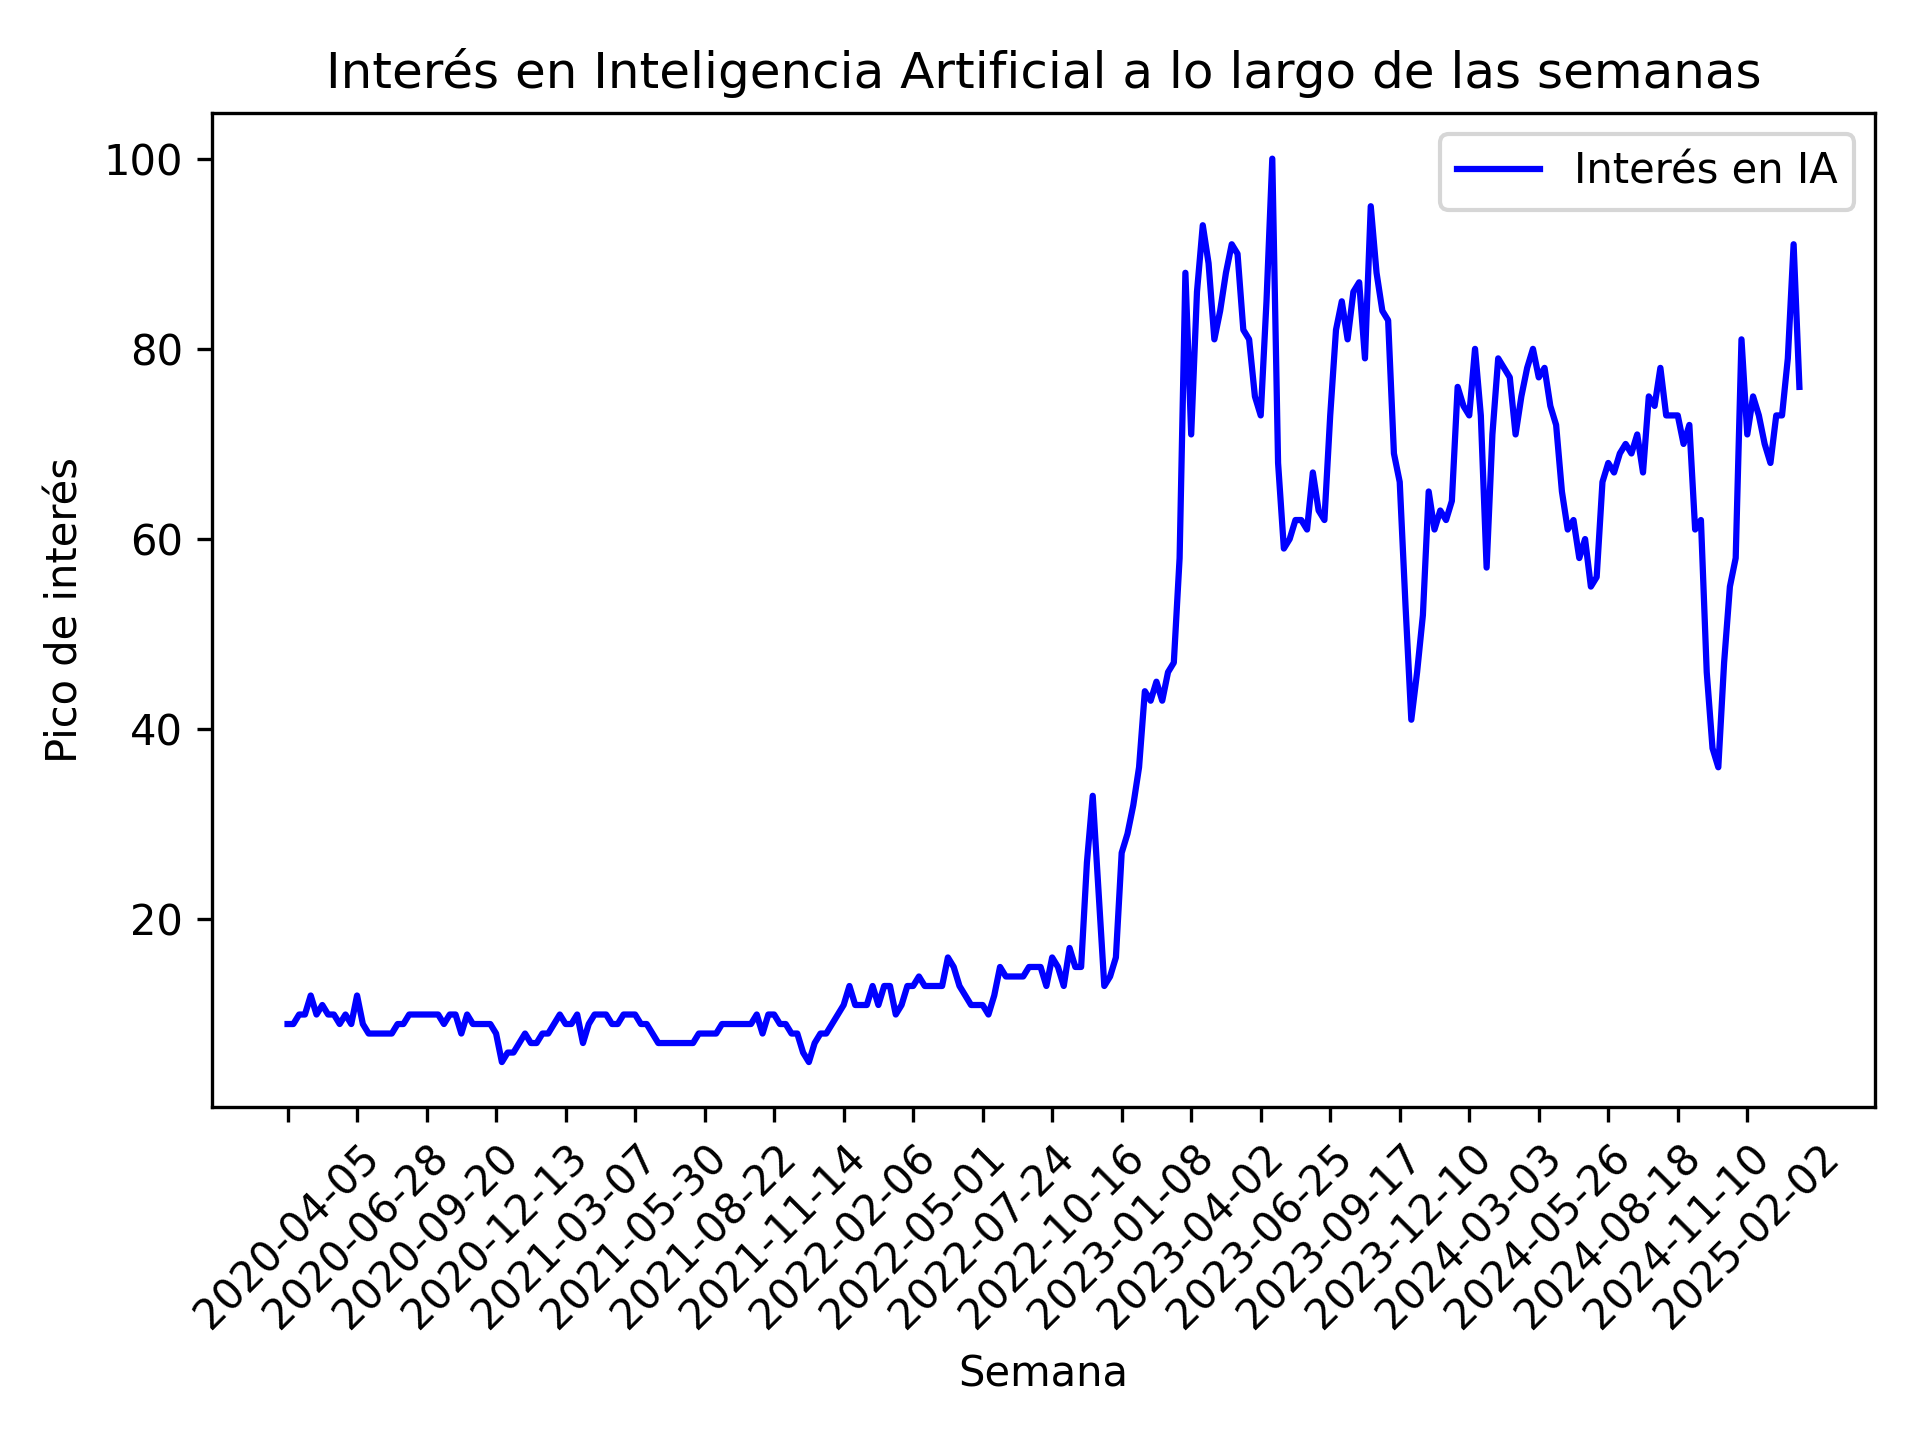
\includegraphics[width=0.7\textwidth]{excels/introduccion/interes_en_ia.png}
   \caption{Evolución de la inteligencia artificial a lo largo de las semanas}
   \label{fig:interes_en_inteligencia_artificial}
\end{figure}



Este progreso ha sido posible gracias a los avances en redes neuronales convolucionales, que han revolucionado la capacidad de los sistemas para detectar y clasificar objetos en imágenes y vídeos con una precisión y velocidad antes inalcanzables.

Para hacer frente a las exigencias computacionales de estas tecnologías, la industria ha desarrollado aceleradores hardware especializados en procesamiento de inteligencia artificial. Entre estos destacan las GPUs (Graphics Processing Unit), las TPUs (Tensor Processing Unit) y los DLA (Deep Learning Accelerator). Estos dispositivos, optimizados para operaciones de inferencia, han sido fundamentales para implementar sistemas de visión artificial capaces de procesar información visual en tiempo real, permitiendo su aplicación en entornos que requieren respuestas inmediatas.





\section{Motivaci\'on}

????? ????????????? ????????????? ????????????? ????????????? ????????????? 

\section{Objetivos}

????? ????????????? ????????????? ????????????? ????????????? ?????????????

\section{Estructura de la memoria}

????? ????????????? ????????????? ????????????? ????????????? ????????????? 

%\section{Notes bibliografiques} %%%%% Opcional

%????? ????????????? ????????????? ????????????? ????????????? ?????????????

%%%%%%%%%%%%%%%%%%%%%%%%%%%%%%%%%%%%%%%%%%%%%%%%%%%%%%%%%%%%%%%%%%%%%%%%%%%%%%%
%                         CAPITOLS (tants com calga)                          %
%%%%%%%%%%%%%%%%%%%%%%%%%%%%%%%%%%%%%%%%%%%%%%%%%%%%%%%%%%%%%%%%%%%%%%%%%%%%%%%

\chapter{Estado del arte}

????? ????????????? ????????????? ????????????? ????????????? ?????????????

\section{Redes neuronales convolucionales}
Evolución de las redes neuronales convolucionales desde region based proposals (two stage regression) a single shot detector (one stage regression), YOLO y por último YOLO11. Hablar de las métricas de evaluación de los modelos, precisión, recall, mAP50 y mAP50-95.
\section{Aceleradores de procesamiento gráfico}
Evolución de los aceleradores de procesamiento gráfico desde la GPU, hasta los dispositivos de bajo consumo en la serie Jetson de NVIDIA.

\section{Seguimiento de objetos en tiempo real}
Explicación de como funcionan los algoritmos de multi-object tracking (MOT) en tiempo real, filtro de Kalman hasta BYTETrack.

\section{SAHI}
Explicación de la técnica de Slicing Aided Hyper Inference, como se utiliza para mejorar la precisión de los modelos de detección de objetos y como se aplica en este trabajo.

\chapter{Análisis del problema}

????? ????????????? ????????????? ????????????? ????????????? ????????????? 

\chapter{Diseño e implementación de la solución}
En este capítulo se explicará la solución propuesta, como se ha diseñado y como se ha implementado.

\section{Descripción del sistema}

Descripción del sistema de visión artificial propuesto, como se ha diseñado y como se ha implementado.

\section{Diseño de las etapas del sistema}

Descripción de las etapas del sistema, como se han diseñado y como se han implementado.

Etapas del sistema:
\begin{itemize}
   \item \textbf{Captura de imágenes:} Descripción de la etapa de captura de imágenes, como se ha diseñado y como se ha implementado.
   \item \textbf{Inferencia:} Descripción de la etapa de inferencia, como se ha diseñado y como se ha implementado.
   \item \textbf{Seguimiento:} Descripción de la etapa de seguimiento, como se ha diseñado y como se ha implementado.
   \item \textbf{Escritura de resultados:} Descripción de la etapa de escritura de resultados, como se ha diseñado y como se ha implementado.
\end{itemize}

\section{Segmentación de las etapas del sistema}

Tipos de segmentación de las etapas del sistema:

\begin{itemize}
   \item \textbf{No segmentada:} Secuencial
   \item \textbf{Segmentación basada en hilos:} Cada etapa del sistema se ejecuta en un hilo diferente.
   \item \textbf{Segmentación basada en procesos:} Cada etapa del sistema se ejecuta en un proceso diferente.
   \item \textbf{Segmentación basada en hardware:} La etapa de inferencia se ejecuta en GPU, DLA0 y DLA1.
   \item \textbf{Segmentación basada en procesos con memoria compartida:} Cada etapa del sistema se ejecuta en un proceso diferente, pero comparten la memoria.
\end{itemize}
    


\chapter{Análisis de la solución}

En este capítulo se analizará la solución propuesta variando los parámetros posibles

\section{Variación de los parámetros}
Explicación de los parámetros que se pueden variar en la solución propuesta y su efecto en el rendimiento del sistema.

------PRUEBA--------


\begin{table}[h]
   \centering
   \resizebox{\textwidth}{!}{ % Ajusta el ancho al tamaño de la página
   \pgfplotstabletypeset[
       col sep=comma, % Definir separador de columnas (por si el CSV usa comas)
       header=true,    % Usar la primera línea como encabezado
       columns={Model, IoU, CPU_Inference, GPU_Inference, DLA_Inference, CPU_Power, GPU_Power, DLA_Power, CPU_Energy, GPU_Energy, DLA_Energy}, % Seleccionar columnas a mostrar
       display columns/0/.style={column name=Model, string type}, % Formato de la columna 'Model'
       display columns/1/.style={column name=IoU}, % Formato de la columna 'IoU'
       display columns/2/.style={column name=CPU\_Inference, column type={|c|}}, % Estilo para columnas de inferencia
       display columns/3/.style={column name=GPU\_Inference, column type={|c|}}, 
       display columns/4/.style={column name=DLA\_Inference, column type={|c|}},
       display columns/5/.style={column name=CPU\_Power, column type={|c|}}, % Estilo para columnas de potencia
       display columns/6/.style={column name=GPU\_Power, column type={|c|}},
       display columns/7/.style={column name=DLA\_Power, column type={|c|}},
       display columns/8/.style={column name=CPU\_Energy, column type={|c|}}, % Estilo para columnas de energía
       display columns/9/.style={column name=GPU\_Energy, column type={|c|}},
       display columns/10/.style={column name=DLA\_Energy, column type={|c|}},
       every head row/.style={before row=\toprule, after row=\midrule}, % Reglas horizontales en el encabezado
       every last row/.style={after row=\bottomrule}, % Reglas horizontales al final
       every column/.style={sci zerofill}, % Opcional, ajusta el formato numérico
       empty cells with={NaN} % Reemplaza celdas vacías o con guiones por NaN
   ]{excels/model_comparasion.csv} % Aquí pones la ruta del archivo CSV
   }
   \caption{Comparación de modelos en términos de inferencia, consumo de energía y potencia.}
   \label{tab:model_comparasion}
\end{table}



------PRUEBA--------



\section{Tipo de segmentación}
En esta sección se analizará el rendimiento de la solución propuesta variando el tipo de segmentación de las etapas del sistema con gráficas y tablas.

\section{Talla del modelo}
En esta sección se analizará el rendimiento de la solución propuesta variando la talla del modelo de detección de objetos con gráficas y tablas.

\section{Precisión del modelo}
En esta sección se analizará el rendimiento de la solución propuesta variando la precisión del modelo de detección de objetos con gráficas y tablas.

\section{Modo de energía y cores de la CPU}
En esta sección se analizará el rendimiento de la solución propuesta variando el modo de energía del dispositivo y el número de cores de la CPU con gráficas y tablas.

\section{Tamaño de la imagen}
En esta sección se analizará el rendimiento de la solución propuesta variando el tamaño de la imagen de entrada del modelo con la técnica de Slicing Aided Hyper Inference (SAHI) con gráficas y tablas.

\chapter{Prueba de concepto}
Aqui se explicará la implementación de la solución propuesta en el entorno de producción con la cinta transportadora.

\section{Construcción del entorno}

\section{Instalación del entorno}






????? ????????????? ????????????? ????????????? ????????????? ?????????????


%%%%%%%%%%%%%%%%%%%%%%%%%%%%%%%%%%%%%%%%%%%%%%%%%%%%%%%%%%%%%%%%%%%%%%%%%%%%%%%
%                                 CONCLUSIONS                                 %
%%%%%%%%%%%%%%%%%%%%%%%%%%%%%%%%%%%%%%%%%%%%%%%%%%%%%%%%%%%%%%%%%%%%%%%%%%%%%%%

\chapter{Conclusiones}

????? ????????????? ????????????? ????????????? ????????????? ????????????? 

%%%%%%%%%%%%%%%%%%%%%%%%%%%%%%%%%%%%%%%%%%%%%%%%%%%%%%%%%%%%%%%%%%%%%%%%%%%%%%%
%                                BIBLIOGRAFIA                                 %
%%%%%%%%%%%%%%%%%%%%%%%%%%%%%%%%%%%%%%%%%%%%%%%%%%%%%%%%%%%%%%%%%%%%%%%%%%%%%%%

\begin{thebibliography}{10}

%%%%%%%%%%%%%%%%%%%%%%%%%%%%%%%%%%%%%%%%%%%%%%%%%%%%%%%%%%%%%%%%%%%%%%%%%%%%%%%
% MODEL D'ARTICLE                                                             %
%%%%%%%%%%%%%%%%%%%%%%%%%%%%%%%%%%%%%%%%%%%%%%%%%%%%%%%%%%%%%%%%%%%%%%%%%%%%%%%
\bibitem{light}
   Jennifer~S. Light.
   \newblock When computers were women.
   \newblock \textit{Technology and Culture}, 40:3:455--483, juliol, 1999.

%%%%%%%%%%%%%%%%%%%%%%%%%%%%%%%%%%%%%%%%%%%%%%%%%%%%%%%%%%%%%%%%%%%%%%%%%%%%%%%
% MODEL DE LLIBRE                                                             %
%%%%%%%%%%%%%%%%%%%%%%%%%%%%%%%%%%%%%%%%%%%%%%%%%%%%%%%%%%%%%%%%%%%%%%%%%%%%%%%
\bibitem{ifrah}
   Georges Ifrah.
   \newblock \textit{Historia universal de las cifras}.
   \newblock Espasa Calpe, S.A., Madrid, sisena edició, 2008.

%%%%%%%%%%%%%%%%%%%%%%%%%%%%%%%%%%%%%%%%%%%%%%%%%%%%%%%%%%%%%%%%%%%%%%%%%%%%%%%
% MODEL D'URL                                                                 %
%%%%%%%%%%%%%%%%%%%%%%%%%%%%%%%%%%%%%%%%%%%%%%%%%%%%%%%%%%%%%%%%%%%%%%%%%%%%%%%
\bibitem{WAR}
   Comunicat de premsa del Departament de la Guerra, 
   emés el 16 de febrer de 1946. 
   \newblock Consultat a 
   \url{http://americanhistory.si.edu/comphist/pr1.pdf}.

\end{thebibliography}
\cleardoublepage

%%%%%%%%%%%%%%%%%%%%%%%%%%%%%%%%%%%%%%%%%%%%%%%%%%%%%%%%%%%%%%%%%%%%%%%%%%%%%%%
%                           APÈNDIXS  (Si n'hi ha!)                           %
%%%%%%%%%%%%%%%%%%%%%%%%%%%%%%%%%%%%%%%%%%%%%%%%%%%%%%%%%%%%%%%%%%%%%%%%%%%%%%%

\APPENDIX

%%%%%%%%%%%%%%%%%%%%%%%%%%%%%%%%%%%%%%%%%%%%%%%%%%%%%%%%%%%%%%%%%%%%%%%%%%%%%%%
%                         LA CONFIGURACIO DEL SISTEMA                         %
%%%%%%%%%%%%%%%%%%%%%%%%%%%%%%%%%%%%%%%%%%%%%%%%%%%%%%%%%%%%%%%%%%%%%%%%%%%%%%%

\chapter{Configuración del sistema}

????? ????????????? ????????????? ????????????? ????????????? ?????????????

\section{Fase de inicialitzación}

????? ????????????? ????????????? ????????????? ????????????? ?????????????

\section{Identificación de dispositivos}

????? ????????????? ????????????? ????????????? ????????????? ?????????????

%%%%%%%%%%%%%%%%%%%%%%%%%%%%%%%%%%%%%%%%%%%%%%%%%%%%%%%%%%%%%%%%%%%%%%%%%%%%%%%
%                               ALTRES  APÈNDIXS                              %
%%%%%%%%%%%%%%%%%%%%%%%%%%%%%%%%%%%%%%%%%%%%%%%%%%%%%%%%%%%%%%%%%%%%%%%%%%%%%%%


\chapter{??? ???????????? ????}

????? ????????????? ????????????? ????????????? ????????????? ????????????? 



%%%%%%%%%%%%%%%%%%%%%%%%%%%%%%%%%%%%%%%%%%%%%%%%%%%%%%%%%%%%%%%%%%%%%%%%%%%%%%%
%                              FI DEL DOCUMENT                                %
%%%%%%%%%%%%%%%%%%%%%%%%%%%%%%%%%%%%%%%%%%%%%%%%%%%%%%%%%%%%%%%%%%%%%%%%%%%%%%%

\end{document}
